\documentclass[10pt,aspectratio=169]{beamer}

\usepackage[utf8]{inputenc}
\usepackage[T1]{fontenc}
\usepackage[spanish]{babel}
\usepackage{lmodern}
\usepackage{xcolor}
\usepackage{graphicx}
\usepackage{booktabs}
\usepackage{tabularx}
\usepackage{hyperref}
\usepackage{tikz}
\usetikzlibrary{arrows.meta,positioning}

\definecolor{tsgreen}{HTML}{14532D}
\definecolor{tslight}{HTML}{F4F6F8}
\definecolor{tsaccent}{HTML}{D4AC0D}
\graphicspath{{presentacion/assets/}{assets/}}

\usetheme{Madrid}
\usecolortheme{default}
\setbeamertemplate{navigation symbols}{}
\setbeamercolor{structure}{fg=tsgreen}
\setbeamercolor{frametitle}{fg=white,bg=tsgreen}
\setbeamercolor{title}{fg=white,bg=tsgreen}
\setbeamercolor{block title}{fg=white,bg=tsgreen}
\setbeamercolor{block body}{bg=tslight}

\title[TurismoSemántico]{TurismoSemántico}
\subtitle{Plataforma inteligente del patrimonio cultural de España}
\author{Sergio Alves Martín}
\institute{Modelado Semántico de la Web}
\date{Mayo de 2026}

\begin{document}

\begin{frame}
  \titlepage{}
  \vspace{-0.35cm}
  \centering
  \footnotesize
  \href{https://github.com/SergioAlvesMar5/ProjectoFinal_MSW_TurismoSemantico}{Repositorio GitHub}
\end{frame}

\begin{frame}{Dominio y objetivo}
  \begin{block}{Problema}
    La información turística y patrimonial está repartida entre fuentes heterogéneas:
    datos semánticos, puntos geoespaciales y servicios contextuales.
  \end{block}
  \begin{itemize}
    \item Dominio: turismo cultural y patrimonio español.
    \item Objetivo: integrar datos abiertos en una app web explorable.
    \item Enfoque semántico: entidades enlazables, RDF/OWL, SPARQL y reutilización.
  \end{itemize}
\end{frame}

\begin{frame}{Fuentes abiertas}
  \small
  \begin{tabularx}{\textwidth}{p{2.5cm}p{2.4cm}X}
    \toprule
    Fuente & Formato & Uso \\
    \midrule
    Wikidata & SPARQL/JSON & Sitios UNESCO, museos, ciudades, descripciones, imágenes e IDs Q. \\
    OpenStreetMap & OSM JSON & Monumentos, castillos, museos y POIs por ciudad con Overpass y Nominatim. \\
    Open-Meteo & REST JSON & Clima actual y previsión por coordenadas. \\
    Anthropic & REST JSON & Chatbot RAG opcional; si no hay clave, respuesta local. \\
    \bottomrule
  \end{tabularx}
\end{frame}

\begin{frame}{Pipeline de datos}
  \centering
  \begin{tikzpicture}[
    node distance=0.8cm,
    box/.style={draw, rounded corners, fill=tslight, minimum width=2.25cm, minimum height=0.75cm, align=center},
    arrow/.style={-{Latex[length=2.6mm]}, thick, draw=tsgreen}
  ]
    \node[box] (extract) {Extracción\\SPARQL/REST};
    \node[box, right=of extract] (clean) {Normalización\\tipos/textos};
    \node[box, right=of clean] (merge) {Fusión\\deduplicación};
    \node[box, right=of merge] (rdf) {RDF/OWL\\Turtle};
    \node[box, right=of rdf] (emb) {Embeddings\\ChromaDB};
    \path[arrow] (extract) -- (clean);
    \path[arrow] (clean) -- (merge);
    \path[arrow] (merge) -- (rdf);
    \path[arrow] (rdf) -- (emb);
  \end{tikzpicture}
  \vspace{0.55cm}
  \begin{itemize}
    \item Caché local en \texttt{data/destinos.json}.
    \item Grafo exportado como \texttt{data/grafo.ttl}.
    \item Fallback TF-IDF si el modelo de embeddings no está disponible.
  \end{itemize}
\end{frame}

\begin{frame}{Modelo semántico}
  \begin{columns}
    \column{0.52\textwidth}
    \begin{itemize}
      \item Ontología propia: \texttt{ts:Destino}, \texttt{ts:Museo}, \texttt{ts:Castillo}, \texttt{ts:PatrimonioUNESCO}.
      \item Propiedades: nombre, descripción, latitud, longitud, imagen, Wikidata ID.
      \item Enlace externo con \texttt{owl:sameAs} hacia Wikidata.
    \end{itemize}
    \column{0.42\textwidth}
    \begin{block}{Evidencia}
      \begin{itemize}
        \item 105 destinos.
        \item 946 tripletas RDF.
        \item Shapes SHACL para nombre, coordenadas y año UNESCO.
      \end{itemize}
    \end{block}
  \end{columns}
\end{frame}

\begin{frame}{Arquitectura}
  \begin{itemize}
    \item Frontend: HTML/CSS/JavaScript, Leaflet para mapa y D3.js para grafo.
    \item Backend: Flask con API REST.
    \item Pipeline: módulos separados para Wikidata, OSM, clima, RDF y embeddings.
    \item Persistencia: JSON, Turtle y ChromaDB.
    \item Integración externa: SPARQL, Overpass, Nominatim, Open-Meteo y LLM opcional.
  \end{itemize}
\end{frame}

\begin{frame}{Funcionalidades}
  \begin{enumerate}
    \item Mapa cultural con filtros por tipo y detalle del destino.
    \item Búsqueda de POIs OSM por ciudad.
    \item Buscador semántico con similitud y NER.
    \item Chatbot RAG con fuentes recuperadas.
    \item Visualización del grafo RDF y descarga Turtle.
    \item Consola SPARQL local con consultas de ejemplo.
  \end{enumerate}
\end{frame}

\begin{frame}{Interfaz: mapa cultural}
  \centering
  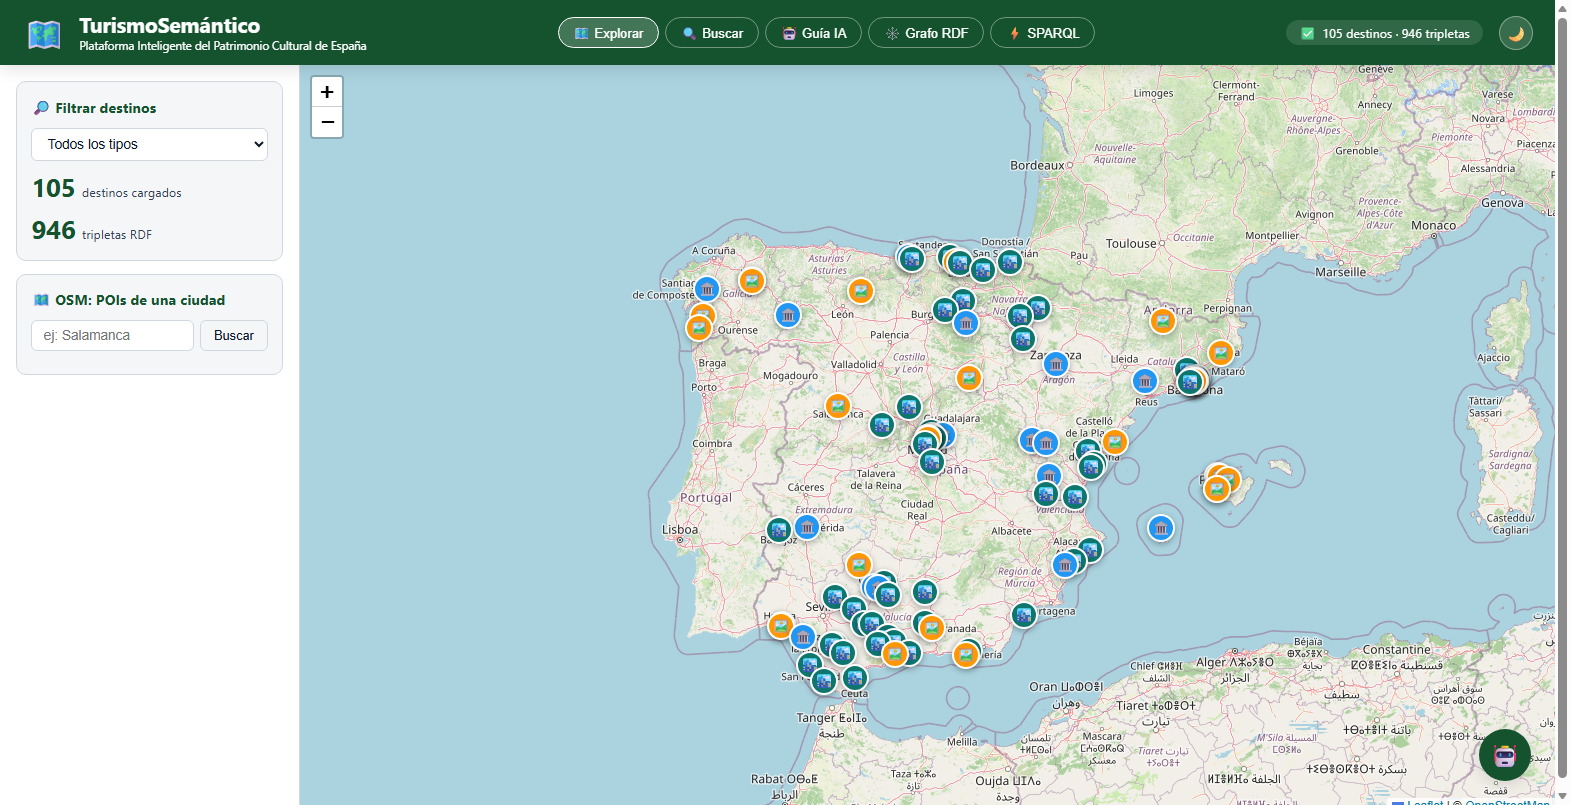
\includegraphics[width=0.96\textwidth,height=0.74\textheight,keepaspectratio]{app-mapa.png}
  \vspace{0.15cm}

  \footnotesize Mapa Leaflet con filtros por tipo, estado de carga y marcadores geográficos.
\end{frame}

\begin{frame}{Interfaz: búsqueda y guía IA}
  \begin{columns}[T,onlytextwidth]
    \column{0.49\textwidth}
      \centering
      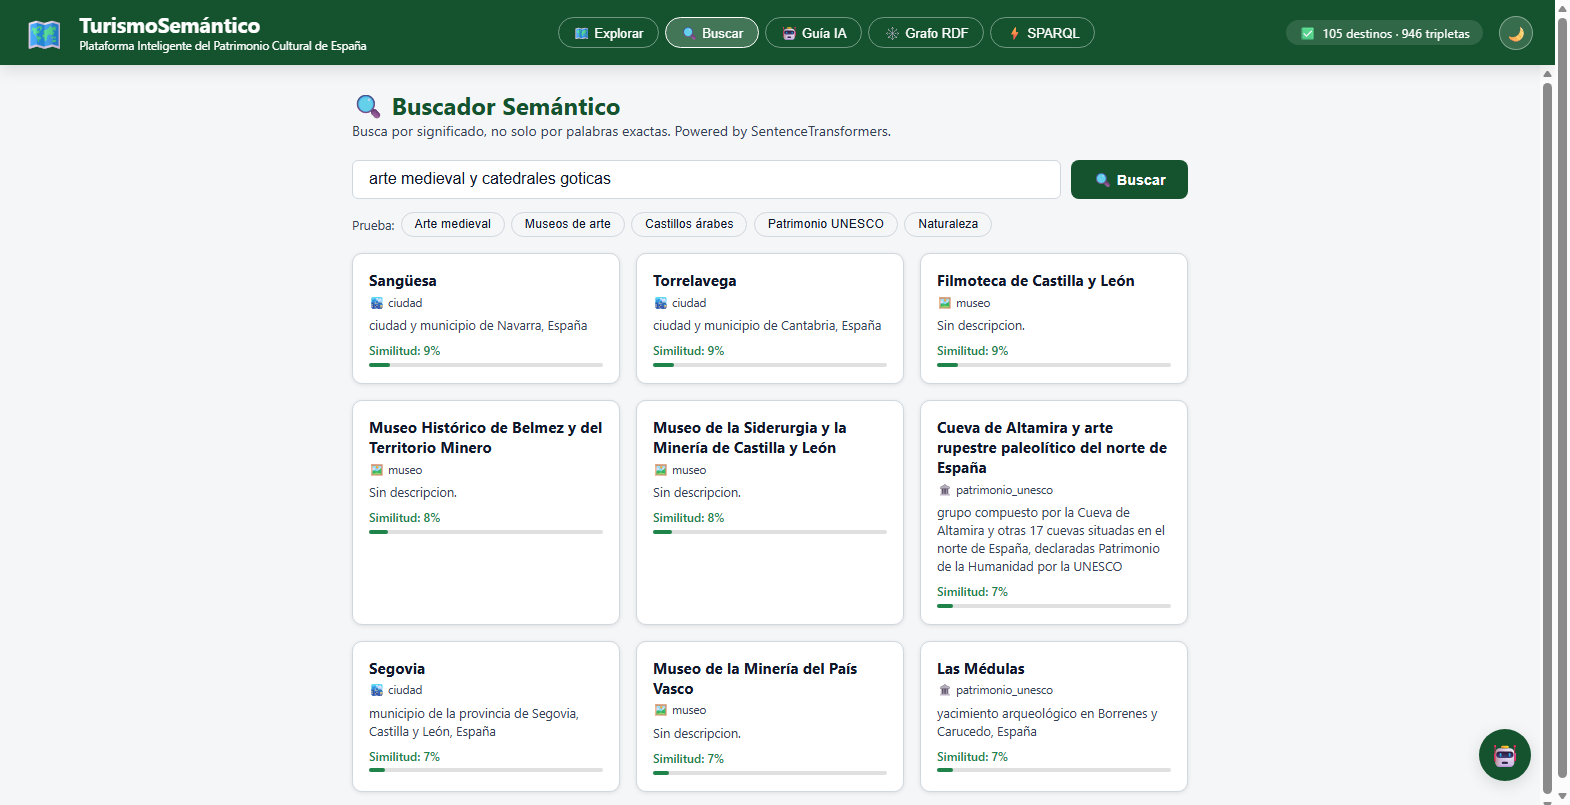
\includegraphics[width=\textwidth,height=0.61\textheight,keepaspectratio]{app-busqueda.png}

      \footnotesize Búsqueda semántica con resultados y similitud.
    \column{0.49\textwidth}
      \centering
      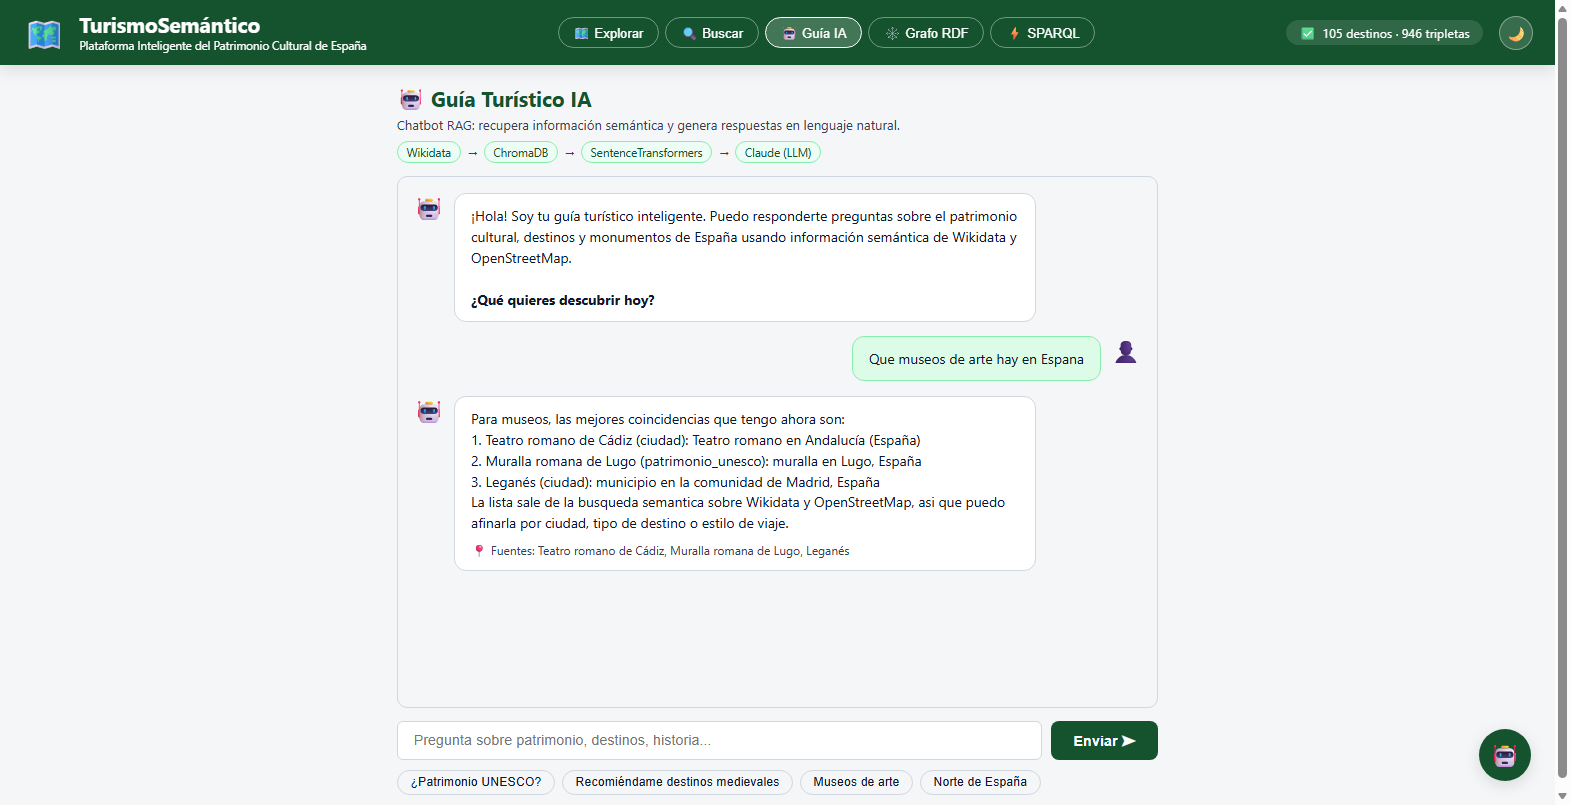
\includegraphics[width=\textwidth,height=0.61\textheight,keepaspectratio]{app-chat.png}

      \footnotesize Chatbot RAG con fuentes recuperadas.
  \end{columns}
\end{frame}

\begin{frame}{Interfaz: grafo RDF}
  \centering
  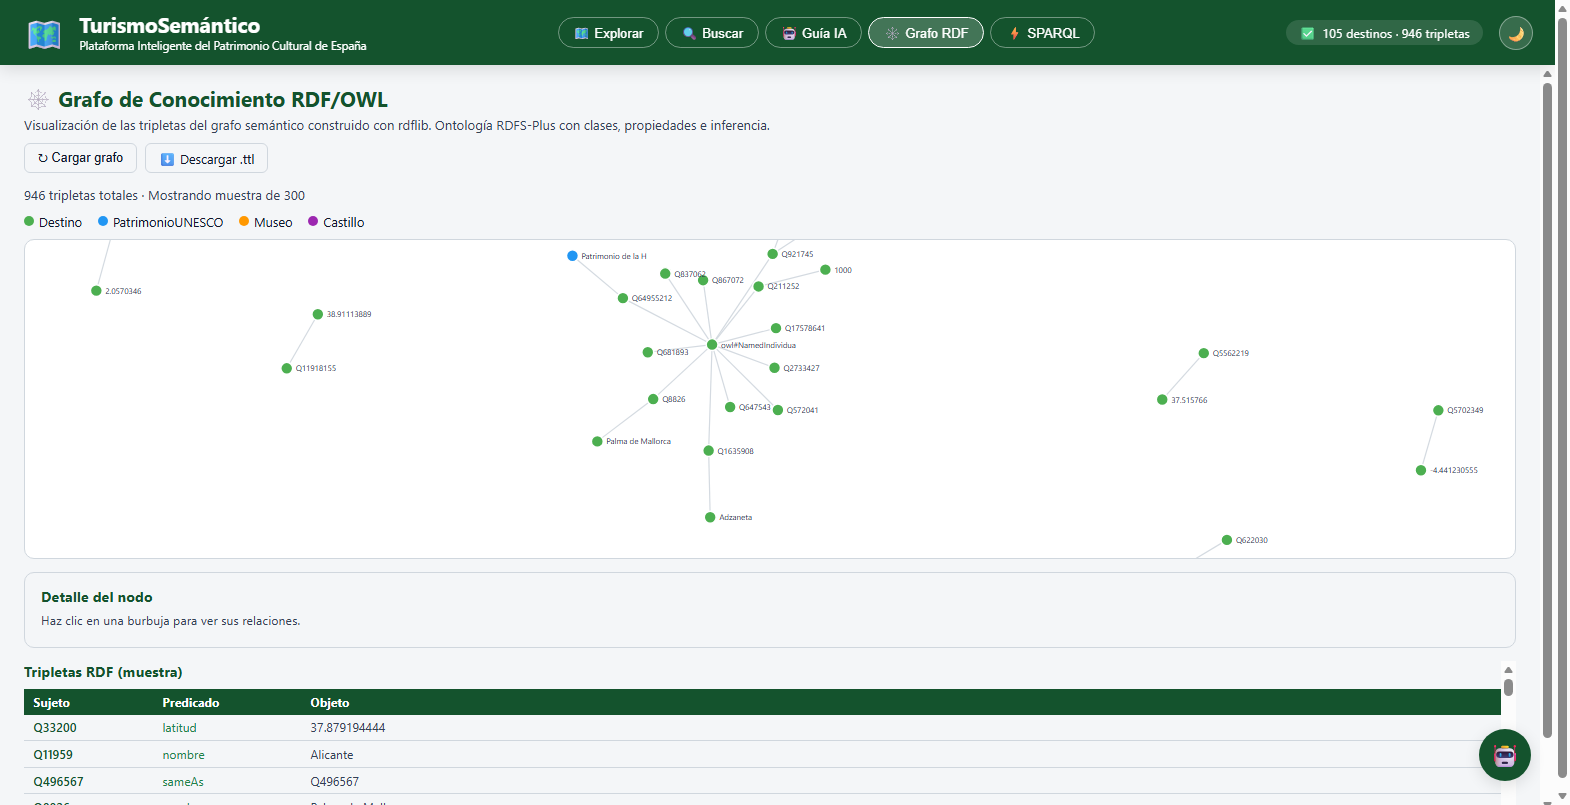
\includegraphics[width=0.96\textwidth,height=0.74\textheight,keepaspectratio]{app-grafo.png}
  \vspace{0.15cm}

  \footnotesize Visualización D3 del grafo, tabla de tripletas y descarga Turtle.
\end{frame}

\begin{frame}{Accesibilidad y robustez}
  \begin{itemize}
    \item Interfaz responsive, modo claro/oscuro y foco visible.
    \item Etiquetas ARIA y regiones \texttt{aria-live} para feedback de carga.
    \item Validación de parámetros REST y salida segura en el frontend.
    \item Degradación controlada: caché, TF-IDF, respuesta local y OSM en segundo plano.
  \end{itemize}
\end{frame}

\begin{frame}{Demo en directo}
  \centering
  \vspace{0.4cm}
  {\Large Abrir la aplicación local para la demostración}

  \vspace{0.45cm}
  \href{http://127.0.0.1:5000}{\beamergotobutton{\Large Abrir demo local}}

  \vspace{0.55cm}
  \begin{block}{Flujo de demo}
    Mapa y filtros \(\rightarrow\) búsqueda semántica \(\rightarrow\) guía IA \(\rightarrow\) grafo RDF \(\rightarrow\) SPARQL.
  \end{block}

  \vfill
\end{frame}

\end{document}
